
\documentclass{article}
\usepackage{amsmath}
\usepackage{caption}
\usepackage{placeins}
\usepackage{graphicx}
\usepackage{subcaption}
\usepackage{tikz}
%\usepackage[active,tightpage]{preview}
\usepackage{natbib}
\bibpunct{(}{)}{,}{a}{}{;} 
\usepackage{url}
\usepackage{nth}
% for the d in integrals
\newcommand{\dd}{\; \mathrm{d}}

\usepackage[top=2in, bottom=1.5in, left=1in, right=1in]{geometry}
\usepackage{setspace}
% matrix numbering
\usepackage{trivfloat}
\trivfloat{matrix}
\floatstyle{plaintop}
    \restylefloat{matrix}
\AtBeginDocument{\numberwithin{matrix}{section}}
% end preamble
%-------------------------------------------------------

\begin{document}

\title{Renewal and stability in populations structured by remaining
years of life}
\author{Tim Riffe \\ University of California, Berkeley}
\maketitle

\begin{abstract}
A unisex model of population renewal for populations structured by
thanatological age is presented in both continuous and discrete form. Various
stable and transient properties populations are compared and related when viewed
by chronological versus thanatological age. Results from the two age perspectives are conformable if the starting
population is stable, but are otherwise divergent.
\end{abstract}

*This is a work in progress. All findings are preliminary at this time, so
please don't cite without permission of the author.
\vspace{2em}

\onehalfspacing
All demographic forces vary over age in known and regular ways. Information on
such forces, along with the size and age structure of a population allows the
demographer to make predictions about the future size and structure of a population. In this
paper, I explore some formal demographic consequences of a particular
redefinition of age. Instead of counting age as the time passed between birth and the present (or
some other moment), consider age as the amount of time left from the present
until death\footnote{This quantity is referred to as \textit{residual} lifetime
in the reliability literaure.}. Individuals in this case move in the same
direction along imaginary life lines, but the reference point for age is now at
the end of the life line instead of at the beginning. For individuals, the
timing of events in life is mirrored exactly between the two definitions of age,
but aggregate patterns differ.

Direct information on the timing of demographic transitions with respect to
death is only available from long-running panel or linked historical data that are few and far between. Some surveys also ask respondents in various ways about
their perceived future lifetime, which may underly those
demographic transitions governed to some degree by volition. The present inquiry
draws only from lifetable-projected remaining lifetime, which
is intended to approximate actual remaining lifetime.
The lifetable methods applied here follow those of \citet{brouard1986structure}
or \citet{miller2001increasing}, which redistribute age-classified counts over
future death times according to a fixed mortality schedule. This allows us to make statements about the remaining lifelines within a current stock of population, under certain assumptions.

Temporal perspectives and rescalings of the lifecourse are abundant in
demography already. It is my view that these efforts have enriched the
discipline by producing new insights and questions much more than they have obscured it by
producing conundrums. Likely some demographic phenomena are best
described as a function of time since birth, and others of time until death,
while still others can be a function of both to some degree. Fertility and
reproduction are plausibly a function of both age perspectives, and the question
of how to partition such forces and events over time is a new conundrum that I
do not tackle here. The model presented here should therefore not be interpreted
as a suggestion for a better way to model or project population, but as an
alternative way to tell the story of population renewal.

Thanatological (counting down towards death) and chronological (counting up
from birth) renewal models, such as the Lotka-Euler renewal model, both
approximate the movement of population stocks over time, but from opposite
vantage points. Specifying a model of thanatological renewal expands the toolbox
available to approach complex temporal population structure. I present a set of
preliminary findings to help understand the implications of temporal structure.

\section*{A lifetable approximation of thanatological age}

A lifetable approach to transforming chronologically classified data into
thanatologically classified data is valid when the given lifetable accurately
describes the future mortality of age-classified population. To make
a projective statement about a current stock of population, one does well to
factor in future changes in mortality, and to allow the trajectory of changes
to vary between ages/cohorts. In the case of a stable population model,
mortality is assumed invariant over time, which means that the same survival
pattern underlies each chronological age class, and we therefore draw from a
single lifetable. Under these conditions, data classified by chronological age
can be decomposed and redistributed into thanatological age classes with a
single mortality pattern. The basic operation is to multiply the probability of
surviving from exact chronological age $a$ to exact age $a+y$,
$\frac{l(a+y)}{l(a)}$, and then dying at exact age $a+y$, $\mu(a+y)$. The
index $y$ in this case means $y$ years in the future. For age 0 this probability
is simply the $d(a)$ column of the lifetable, standardized to sum to 1. For higher ages, simply condition on survival:\footnote{In the reliability literature, our concept of $d(y|a)$ is denoted by \begin{equation} X - t | X > t
\end{equation}
where $X$ is the total lifespan and $t$ is the current chronological age
attained.}

\begin{equation}
\label{eq:vaupel1}
d(y | a) = \mu(a+y)\frac{l(a+y)}{l(a)}
\end{equation}

A convenient discretization of \eqref{eq:vaupel1} is to simply work with the
$d_a$ column of the lifetable (here with single ages):

\begin{equation}
d_{y, a} =  \frac{d_{a+y}+d_{a+y+1}}{L_a + L_{a+1}} \quad\quad \text{,}
\end{equation}

\noindent where $\omega$ is the highest age. One
produces in this way a probability density function over future death times
for each chronological age, $a$, and the $d(y|a)$- weighted average of $y$ for
a given $a$ returns the familiar remaining life expectancy column of the lifetable,
$e(a)$. If $P(a)$ is an chronological age-classified population count,
we can derive $P(y)$, a thanatological age-classified population count, as
follows:

\begin{align}
\label{eq:transform}
P(y) =& \int_0^\infty P(a) d(y | a) \dd a
\end{align}

Since $1 = \int_0^\infty d(y|a) \dd y$ for each $a$,
this density is useful for decomposing data classified by chronological age. For
example, we can break down a population pyramid into thanatological age classes.
Figure~\ref{fig:USdecomp} shows this exercise for 2010 US data, assuming the
2010 period mortality schedule remains constant. When looking from the
chronological age perspective, this decomposition reveals thanatological
heterogeneity, but when viewed from the thanatological perspective
(Figure~\ref{fig:USdecomp}) it reveals chronological age heterogeneity and the
overall thanatological age profile, the future death flow of the current
population.
Figure~\ref{fig:USrecomp} shows this \textit{re}composition for the same 2010
US data.

\begin{figure}[ht!]
	\caption{2010 US population structure}
	\begin{center}
	\begin{subfigure}{.45\textwidth}
		\caption{Chronological age-structure (years lived) decomposed by
		thanatological age (years left).}
		\label{fig:USdecomp}
		\includegraphics[scale=.6]{Figures/US2010Age.pdf}
	\end{subfigure}
	~
	\begin{subfigure}{.45\textwidth}
		\caption{Thanatological age-structure (years left) decomposed by chronological
		age (years lived).}
		\label{fig:USrecomp}
		\includegraphics[scale=.6]{Figures/US2010Thano.pdf}
	\end{subfigure}
	\\
	\small{*Population and mortality data from the HMD.}
	\end{center}
\end{figure}

\citet{brouard1986structure} applied this method to highlight regional
differences in French age structure, at times combining this projective method
with historical stocks. \citet{brouard1989mouvements}, and later
\citet{vaupel2009life}, showed that in stationary populations the chronological
and thanatological age structures are identical, and this provides a
limited basis for comparison between the two perspectives. \citet{wachter2014essential} hints at, and
\citet{vaupel2014stable} elaborates on how to make chronological and
thanatological age structure commensurate under a constant growth rate, $r$.
These results will also follow from the following specification of a
thanatological renewal model.

It bears repeating that lifetable-derived thanatological age structure is probabilistic until after death, since it refers to the future according to an assumed mortality pattern.
As such, Figure~\ref{fig:USrecomp} is projective in nature, a forward-looking
glance at population attrition given the population stock and lifetable of a
particular moment, whereas Figure~\ref{fig:USdecomp} is reflective in nature, since a population's chronological age-structure is mostly the fruit of past fertility, but also migration and to a lesser degree attrition. Note that any count classified by chronological age can be
reclassified in this way, as long as you have a lifetable that plausibly represents the population whose data you wish to reclassify. This means we can derive thanatological fertility rates, $F_y$, by applying \eqref{eq:transform}
to age-classified birth counts, $B_a$, to get $B_y$ and again to
exposure-to-risk, $E_a$ (here we take exposures from all ages), to get $E_y$ and then dividing:

\begin{equation}
f^\star_y = \frac{B_y}{E_y}
\end{equation}

We are interested to use thanatological fertility rates, $F_y$ in
models of population renewal,\footnote{This is probably premature, but helps to
understand the nature and provenance of model components.} rather than to
explicitly study the nature of these rates. Nonetheless it is best not to throw such rates into a model blindly, so we offer a schematic overview of some of their characteristics.
Figure~\ref{fig:FySpaghetti} represents the full variety in
female thanatological period fertility rates that can be found for all years
of data that overlap in the HFD and HMD.\footnote{There are as of this writing
1834 population-years of overlap between the HMD and HFD, including a wide
variety of fertility and mortality combinations.} Figure~\ref{fig:FxSpaghetti} gives ASFR for the same
populations and years as a more familiar reference, but note that both scales
are different! With no indication of particular populations or time series, one
already concludes that period thanatological fertility rates have a
characteristic shape and are not random, erratic or informationless: There is a
pattern to fertility rates by remaining years of life, and it varies over time
and between populations within some range of normality. Thanatological fertility
rates have a wider distribution than do chronological rates. Note that this
spaghetti plot includes both fertility booms and busts, as well as some
mortality crises (1918, WWII). Some patterns to note, but which we do not
separate graphically here, are that the left tail (a gauge of how orphan-prone a
population is) has tended to fall over time. All populations have shown a
rightward shift in both the mean and modal mother's thanatological age at birth
(TAB) over time (that's unambiguously a good thing). Several populations now
show modal TABs of over 60 years. Thanatological total fertility rates (TTFR)
track standard period total fertility rates (PTFR) rather closely, but tend to
be somewhat higher (not shown).

\begin{figure}[h!]
	\caption{Chronological and thantological fertility rates, all 1600
	country-year combinations present in both the HFD and HMD.* Note different x
	and y scales.}
	\label{fig:Fxcompare}
	\begin{center}
	\makebox[\textwidth]{
	\begin{subfigure}{.45\textwidth}
		\caption{Chronological period fertility rates.}
		\label{fig:FxSpaghetti}
		\includegraphics[scale=.45]{Figures/FxSpaghettiDraft.png}
	\end{subfigure}
	~
	\begin{subfigure}{.45\textwidth}
		\caption{Thanatological period fertility rates.}
		\label{fig:FySpaghetti}
		\includegraphics[scale=.45]{Figures/FySpaghettiDraft.png}
	\end{subfigure}
	}
	\\
	\end{center}
	\begin{tiny}
	*AUT, $1951-2010$; BGR, $1947-2009$; BLR, $1964-2009$; CAN, $1921-2007$; 
	CHE, $1932-2011$; CZE, $1950-2011$; DEUTE, $1956-2010$; DEUTNP, $1990-2010$; 
	DEUTW, $1956-2010$; ESP, $1922-2006$; EST, $1959-2010$; FIN, $1939-2009$; 
	FRATNP, $1946-2010$; GBR\_NIR, $1974-2009$; GBR\_NP, $1974-2009$; GBR\_SCO,
	$1945-2009$; GBRTENW, $1938-2009$; HUN, $1950-2009$; IRL, $1955-2009$; JPN, $1947-2009$; 
	LTU, $1959-2010$; NLD, $1950-2009$; NOR, $1967-2009$; PRT, $1940-2009$; 
	RUS, $1959-2010$; SVK, $1950-2009$; SVN, $1983-2009$; SWE, $1891-2010$; 
	TWN, $1976-2010$; UKR, $1959-2006$; USA, $1933-2010$
	\end{tiny}
\end{figure}

In general, such fertility rates will not be palatable for purposes of
projection, unless the demographer believes that their empirical regularity is
somehow stronger than typical ASFR --- an argument we do not make. There may be
alternative ways of defining thanatological fertility rates, for instance by
transforming from a stable population, which would make the resulting model more
conformable with the Lotka renewal model. First let us define the basic model.

\FloatBarrier
\section*{The thanatological renewal model}
For the renewal model that follows, we are most interested in using the kind
of fertility rates shown in Figure~\ref{fig:FySpaghetti}, and we refer to a
unisex population based on female vital rates. In the following, I
explain describe the model in four different ways: as a continuous
model, as a matrix model, with a lifecylcle graph, and intuitively by
appealing to how population pyramids and leaves (described earlier) change over
time. Assuming constant vital rates, the births for the present year are given by
\begin{align}
B(t) =& \int _0^\infty P(y,t)f^\star(y) \dd y = \int _0^\infty P(a,t)f(a) \dd a
\quad\text{,} \intertext{where $a$ indexes chronological age, $y$ indexes
thanatological age, $P(a), P(y)$ are population counts, and $f^\star(y), f(a)$ are
exact specific fertility probabilities (rates), which here are best thought of
as the fertility rates of females born to females. The thanatological integral can
be broken down back in terms of chronological age:} =& \int_{y=0}^\infty
\int_{a=0}^\infty f^\star(y)\frac{P(a,t)d(a+y)}{l(a)} \dd a \dd y \quad\text{,}
\intertext{where $d(a)$ is the continuous lifetable death distribution with
radix of 1, so $d(a)/l(0)$. We can relate the present population to past births
with $P(a,t) = B(t-a)l(a)$:}
\label{eq:ergostep1}
=& \int_{y=0}^\infty \int_{a=0}^\infty f^\star(y) B(t-a)d(a+y)\dd a \dd y
\quad\text{.} \intertext{Eventually-- usually a bit quicker than is the case for
chronological age-- strong ergodicity will assert itself, and $B(t)$ will be related to
$B(t-a)$ according to a constant factor $e^{ra}$, where $r$ is the familiar
intrinsic rate of growth:}
\label{eq:ergostep2}
=& \int_{y=0}^\infty \int_{a=0}^\infty f^\star(y) B(t)e^{-ra}d(a+y)\dd a \dd y
\quad\text{.}
\intertext{Divide out $B(t)$ to get back a familiar-looking renewal equation:}
\label{eq:thanoren}
1 =& \int_{y=0}^\infty \int_{a=0}^\infty f^\star(y) d(a+y)e^{-ra}\dd a \dd y
\quad\text{.}
\end{align}
Now compare this to Lotka's chronological formulation
\begin{equation}
\label{eq:lotka}
1 = \int_{a=0}^\infty f(a)l(a)e^{-ra}\dd a \quad\text{,}
\end{equation}
and note that these are really quite similar, since $\int _{y=0}^\infty
d(a+y)\dd a = l(a)$. For intuition, notice that $l(a)$ is here split
up into pieces of $d(a)$, and imagine a 2D surface of these, where one axis is chronological age and the
other axis is thanatological age. For the chronological case \eqref{eq:lotka},
we multiply chronological age-specific fertility rates over one margin, and for
the thanatological case over the other margin. There is a strong parallel here
with the case of two-sex age-specific fertility rates. As in the case of
divergence between male and female single-sex models, there will always be divergence between
single-sex models under chronological versus thanatological age, unless the
starting population is stable. Even though the modeled population stocks are in
a way commensurable, the rates used here, $f(a)$ versus $f^\star(y)$ are
calculated on the basis of differently distributed denominators $E(a)$ versus $E(y)$.

There are gaps in the above line of development, since the jump from
\eqref{eq:ergostep1} to \eqref{eq:ergostep2} (strong ergodicity) is unproven,
although it is rather intuitive, given the much greater density of connections
within the model; persons from nearly any thanatologcal age\footnote{I say
\textit{nearly} because the very highest thanatological ages tend to be
composed of pre-menarchical females, so these can be thought of as structural
zeros. I am uncertain if it is a record, but it is certainly an extreme case
useful for illustration: Jeanne Calment, who lived to 122, had a daughter at age
22, which means she was about thanatological age 100
(\url{http://en.wikipedia.org/wiki/Jeanne_Calment}). If the lifetable used to
transform to thanatological closes out at age 110+, as is the case with HMD data, then fertility rates for thantological ages 101-110+ would be structural
zeros.} can produce offspring that can have any other thanatological age. In
this sense, the smoothing mechanism at play as the population passes through
time must be much stronger than that for chronological age, at least in most
cases. A further conjecture is that the jump will also hold for the case of weak ergodicity. The mechanisms at play unfold in the same way as those so intuitively described by \citet{arthur1982ergodic}, and said proof may apply here without further modification. A proof of the uniqueness of the solution to \eqref{eq:thanoren} is given in Appendix~\ref{app:A}.

Once one finds $r$ from \eqref{eq:thanoren}, other familiar stable population
parameters can be calculated. For instance, we may calculate the mean
thanatological generation time, $T^y$:
\begin{equation}
\label{eq:Ty}
 T^y =  \frac{\int _{y=0}^\infty \int _{a=y}^\infty y e^{-ra} d(a) f^\star(y) \dd a
\dd y}{\int _{y=0}^\infty \int _{a=y}^\infty e^{-ra} d(a) f^\star(y) \dd a \dd
y} \quad \text{.}
\end{equation}
Literally, this is the mean of the remaining lifespans of new mothers in the
stable population. The net reproduction rate, $R_0$ is related by, e.g.,
\begin{equation}
\label{eq:R0fromTy}
R_0 = e^{r T^y}
\end{equation}
The birth rate, $b$, is given by
\begin{equation}
\label{eq:eybrate}
b = \frac{1}{\int _{y=0}^\infty \int _{a=y}^\infty e^{-ra} d(a) \dd a
\quad\text{.} \dd y}
\end{equation}
The stable thanatological age structure, $c_y$, is the
proportion of the stable population with remaining years to live $y$:
\begin{equation}
\label{eq:cy}
c(y) = b \int _{a=y}^\infty e^{-ra} d(a) \dd a \quad\text{.}
\end{equation}
We already knew that when $r = 0$ and $y = a$, that $c(a)=c(y)$
\citep{vaupel2009life}, and now we can arrive at the same conclusion directly
by equating the chronological and thanatological renewal equations. For
small non-zero magnitude values of $r$ and survival patterns typical of humans, it is also the
case that $c(y|r)\approx c(a|-r)$. The relationship is asymptotically exact as
$r$ approaches zero. Other findings regarding stable age structure will be
presented in a future version of this paper. Further stable population
quantities may be estimated by similarly translating the various common definitions (e.g.,
in the glossary of \citet{coale1972growth}) to the present perspective. We will
focus on the main model rather than on these.

The thanatological renewal model is coherent, but these ideas may take some time
to gestate before accepting that it is also a valid description of how
populations renew. What should one imagine under the model of thanatological
population renewal? A useful mnemonic bases itself on Figures~\ref{fig:USdecomp}
and \ref{fig:USrecomp}. In the chronological age-structured model, new
generations appear at the bottom of the pyramid, and move up one rung per year.
All age-classes are subject to attrition, which is spread out over ages and not
readily visible in the pyramid. In the thanatological \textit{leaf}, each birth cohort increments to the population over the whole range of thanatological age
according to $d(a)$, as seen in \eqref{eq:thanoren}, becoming the
shaded layers seen in Figure~\ref{fig:USrecomp}. Each horizontal step is a death
cohort, and these move one step down the pyramid each year without any decrement
(indeed incrementing due to births) until reaching the very bottom. In short,
the locations of increment and decrement, and the direction of movement are all
switched. The chronological and thanatological renewal models are almost
perfectly opposite descriptions of the same two processes.

\section*{The thanatological projection matrix}
These descriptions can be made more explicit, and in some ways more tractable,
by hashing out the projection matrix that corresponds to the thanatological renewal model. As with the
chronological age-structured Leslie matrix, the thanatological projection
matrix, $\textbf{Y}$, is square and of dimension $y \times y$, where $y$ is the number
of remaining-years classifications on which the population is structured. 
The matrix contains elements for survival and elements for fertility. Unlike
Leslie matrices, $\textbf{Y}$ is not sparse, but is instead populated primarily
with non-zero entries. This is an odd notion, to be explained in following.

Of interest is that mortality occurs in only the population class with zero
remaining years of life. Thanatological age 1 in year $t$ moves to 0 in year
$t + 1$. Thus, instead of in the subdiagonal, we place survival in the
superdiagonal. All survival values are 1, since there is no decrement until
after living through age 0, and the upper-left corner of this superdiagonal
contains a 0, for full decrement. In the following, I illustrate using a
6$\times$6 matrix. The survival component of $\textbf{Y}$ is organized as in
Matrix~\ref{matrix:Ysurv}. To imagine a lifecycle graph, each age decrements by
one through each lower age in successive order until being absorbed by death
after completing thanatological age zero. This chain unfolds in the opposite
index-direction of survival in the chronological age system.

\begin{matrix}[h!]
\centering
\caption{Survival component of unisex thanatological projection matrix,
$\textbf{Y}$}
\label{matrix:Ysurv}
$\bordermatrix{{e_y } & 0_t & 1_t & 2_t & 3_t & 4_t & 5_t\cr 
                0_{t+1} & 0    &  1   & 0    & 0    & 0    & 0   \cr
                1_{t+1} & 0    &  0   & 1    & 0    & 0    & 0   \cr 
                2_{t+1} & 0    &  0   & 0    & 1    & 0    & 0   \cr 
                3_{t+1} & 0    &  0   & 0    & 0    & 1    & 0   \cr 
                4_{t+1} & 0    &  0   & 0    & 0    & 0    & 1   \cr
                5_{t+1} & 0    &  0   & 0    & 0    & 0    & 0   }$
\end{matrix}

 Fertility inputs to the matrix are derived from single-sex thanatological
 fertility and the lifetable $d_a$ distribution, where $a$ indexes age and is
 equated to $y$ remaining years of life for members just born. Fertility
 in a thanatologically structured population occurs in all but the highest
 remaining years classes, which can be thought of as structural zeros for
 simplicity, as they only contain pre-menarchical females. For our
 $6\times 6$ example, say that fertility is observed in classes 0-4, while the
 final class has no fertility, where $f^\star_y$ indicates the fertility
 probability for class $y$ in the year $t$ entering population (in the matrix
 columns). Each $f^\star_y$ is then distributed out according to $d_a$ with no
 further translation, since the $d_a$ lifetable column already refers to age 0. Thus, the fertility entry in row $m$ and column $n$ of $\textbf{Y}$ will be $f^\star_n \cdot d_m$. We assume that those dying over the course of year
 $t$ (the first column) are exposed to fertility for half of the
 year,\footnote{One might be tempted to not allow for fertility at all for
 females dying in year $t$, but recall that fertility is measured in the moment of
 birth, and not conception.}
 and so discount the fertility entry accordingly. Further, infant mortality, 
 $f^\star_y \cdot d_0$, located in the first row, must also be discounted, since part
 of the mortality will occur in the same year $t$ and the rest in year $t + 1$. 
 The first row of fertility must be further discounted by a factor, $\lambda$,
 in order to account for the fact that infant mortality is higher in the lower Lexis 
 triangle than in the upper: of those infants who die in the first year of life, a proportion equal to
 $\lambda$ do not make it to December \nth{31} of the calendar year in which
 they were born.\footnote{$\lambda$ can be derived directly from death counts
 data classified by Lexis triangles. In the US, $\lambda$ has behaved similarly
 for males and females, falling steadily from around $0.9$ in 1969 to $0.86$
 around 1990, since which time it has steadily risen to around $0.87$. That is
 to say, $\lambda$ has varied, but not drastically. These numbers are just meant to give a
feel for the ranges that $\lambda$ can be expected to receive. If the demographer
 does not have information to derive $\lambda$ directly, ad hoc or semidirect
 methods may be used to assign a reasonable proportion. } The
 fertility component of $\textbf{Y}$ is then composed as in Matrix~\ref{matrix:Yfert}.

\begin{matrix}[h!]
\centering
\caption{Fertility component of unisex thanatological projection matrix,
$\textbf{Y}$}
\label{matrix:Yfert}
$\bordermatrix{
  {e_y } \vspace{.6em}&                0_t  & 1_t  & 2_t  & 3_t  & 4_t  & 5_t\cr 
   0_{t+1} \vspace{.6em}& (1-\lambda) \tfrac{f^\star_0d_0}{2} & (1-\lambda) f^\star_1d_0 & (1-\lambda)
   f^\star_2d_0 & (1-\lambda) f^\star_3d_0 & (1-\lambda) f^\star_4d_0 & 0 \cr 
   1_{t+1} \vspace{.6em}& \tfrac{f^\star_0d_1}{2} & f^\star_1d_1 & f^\star_2d_1 & f^\star_3d_1 & f^\star_4d_1
   & 0   \cr 2_{t+1} \vspace{.6em}& \tfrac{f^\star_0d_2}{2} & f^\star_1d_2 & f^\star_2d_2 & f^\star_3d_2 & f^\star_4d_2
   & 0   \cr 3_{t+1} \vspace{.6em}& \tfrac{f^\star_0d_3}{2} & f^\star_1d_3 & f^\star_2d_3 & f^\star_3d_3 & f^\star_4d_3
   & 0   \cr 4_{t+1} \vspace{.6em}& \tfrac{f^\star_0d_4}{2} & f^\star_1d_4 & f^\star_2d_4 & f^\star_3d_4 & f^\star_4d_4
   & 0   \cr 5_{t+1} \vspace{.6em}& \tfrac{f^\star_0d_5}{2} & f^\star_1d_5 & f^\star_2d_5 & f^\star_3d_5 & f^\star_4d_5
   & 0   }$
\end{matrix}
\FloatBarrier

The survival and fertility components of $\textbf{Y}$ add together elementwise,
thus the full 6$\times$6 matrix is composed as in Matrix~\ref{matrix:Y}.

\begin{matrix}[h!]
\centering
\caption{A full unisex thanatological projection matrix, $\textbf{Y}$} 
\label{matrix:Y}
$\textbf{Y} = \bordermatrix{
  {e_y } \vspace{.6em} & 0_t  & 1_t  & 2_t  & 3_t  & 4_t  & 5_t\cr 
  0_{t+1} \vspace{.6em}&  (1-\lambda) \tfrac{f^\star_0d_0}{2} & (1-\lambda) f^\star_1d_0 + 1 &
  (1-\lambda) f^\star_2d_0 & (1-\lambda) f^\star_3d_0 & (1-\lambda) f^\star_4d_0 & 0 \cr 
    1_{t+1} \vspace{.6em}& \tfrac{f^\star_0d_1}{2} & f^\star_1d_1 & f^\star_2d_1 + 1 & f^\star_3d_1 & f^\star_4d_1 & 0 \cr 
    2_{t+1} \vspace{.6em}& \tfrac{f^\star_0d_2}{2} & f^\star_1d_2 & f^\star_2d_2 & f^\star_3d_2 + 1 & f^\star_4d_2 & 0 \cr 
   3_{t+1} \vspace{.6em}& \tfrac{f^\star_0d_3}{2} & f^\star_1d_3 & f^\star_2d_3 & f^\star_3d_3 & f^\star_4d_3 + 1 & 0 \cr 
   4_{t+1} \vspace{.6em}& \tfrac{f^\star_0d_4}{2} & f^\star_1d_4 & f^\star_2d_4 & f^\star_3d_4 & f^\star_4d_4 & 1 \cr 
   5_{t+1} \vspace{.6em}& \tfrac{f^\star_0d_5}{2} & f^\star_1d_5 & f^\star_2d_5 & f^\star_3d_5 & f^\star_4d_5 & 0 }$
\end{matrix}

Figure~\ref{fig:graph} depicts the projection matrix $\textbf{Y}$ in the form of
a lifecycle graph. In this graph, each thanatological age is a node. Population
members are born into any of the thanatological age classes, and then follow
clockwise around the graph on the thick blue paths in order until finally being
absorbed into death (the node labeled ``X'', not included in the projection matrix). The light gray paths represent fertility. Thse originate from any age class that has a fertility rate greater
than zero, which for this toy matrix are all age classes except the \nth{5}
(highest). The y$^{th}$ age class is subject to the fertility rate $f^\star
(y)$, and these births distribute out to all other age classes according to the
lifetable deaths distribution, $d(a)$. Hence, the rate instensity of a fertility
path is determined by the fertility rate of the origin age, and the probability of dying at the destination age. A fraction of the fertility destined for infant mortality equal
to $lambda$ leads straight to the absorbing state of death. Fertility paths from
the \nth{4} thanatological age class have been highlighted. These correspond
to the fifth column of the example matrix $\textbf{Y}$, plus an additional path
direct to death for the fraction of infant mortality prior to December \nth{31}
in year $t$. Paths that loop back into the same age class simply indicate those
offspring that are destined to die in the same year as their mother. It is
perhaps clearer to see from the density of this graph and by recalling that
thanatological fertility distributions are relatively wide (see
Figure~\ref{fig:FySpaghetti}) that there is a high degree of mixing of
thanatological age within populations via reproduction -- a strong tendency
toward stability.

\begin{figure}
\centering
\caption{The thanatological lifecycle graph}
\label{fig:graph}
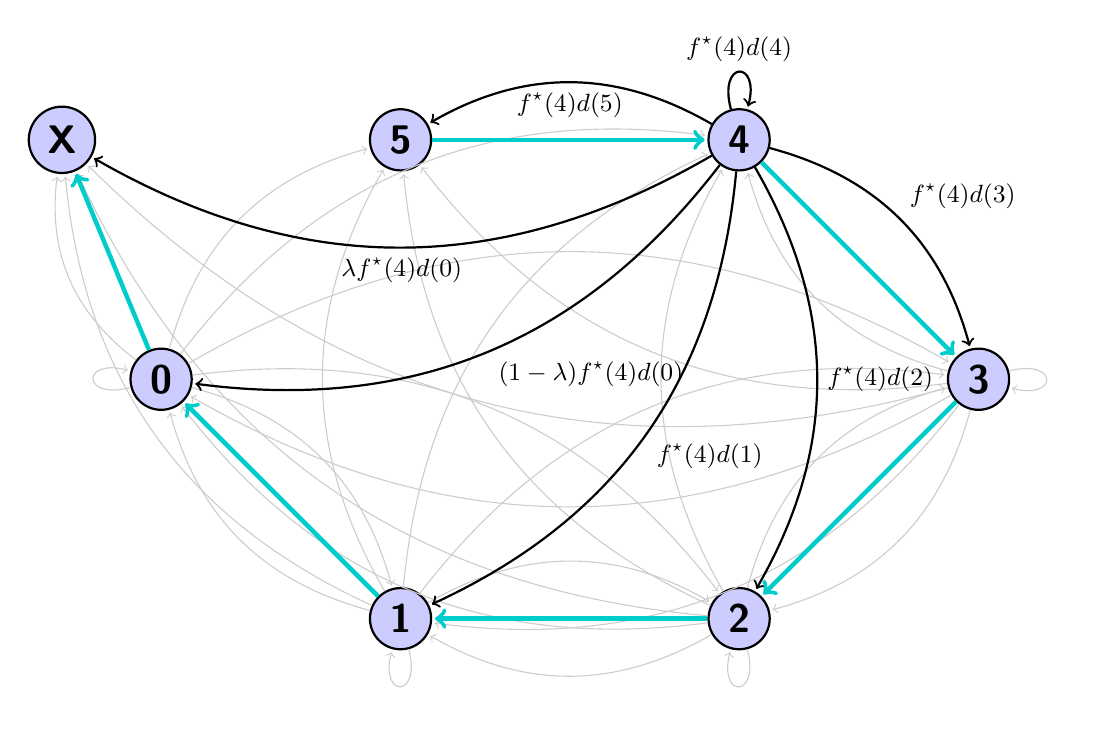
\begin{tikzpicture}[->,shorten >=1pt,auto,node distance=4.3cm,
  thick,main node/.style={circle,fill=blue!20,draw,font=\sffamily\Large\bfseries}]
  \definecolor{gray}{rgb}{0.8,0.8,0.8}
  \definecolor{lightgreen}{rgb}{0,0.8,0.8}
  \node[main node] (0) {0};
  \node[main node] (5) [above right of=0] {5};
  \node[main node] (4) [right of=5] {4};
  \node[main node] (3) [below right of=4] {3};
  \node[main node] (2) [below left of=3] {2};
  \node[main node] (1) [left of=2] {1};
  \node[main node] (X) [left of = 5] {X};

  \path[every node/.style={font=\sffamily\small},draw=gray,thin]
    (3) edge [bend left] node {} (5)
        edge [bend left] node {} (4)
        edge [bend left] node {} (2)
        edge [bend left] node {} (1)
        edge [bend left] node {} (0)  
        edge [bend left] node {} (X)
        edge [loop right] node {} (3) 
    (2) edge [bend left] node {} (5)
        edge [bend left] node {} (4)
        edge [bend left] node {} (3)
        edge [bend left] node {} (1)
        edge [bend left] node {} (0)     
        edge [loop below] node {} (2) 
        edge [bend left] node {} (X)
    (1) edge [bend left] node {} (5)
        edge [bend left] node {} (4)
        edge [bend left] node {} (3)
        edge [bend left] node {} (2)
        edge [bend left] node {} (0)    
        edge [loop below] node {} (1) 
        edge [bend left] node {} (X)
    (0) edge [bend left] node {} (5)
        edge [bend left] node {} (4)
        edge [bend left] node {} (3)
        edge [bend left] node {} (2)
        edge [bend left] node {} (1)
        edge [loop left] node {} (0) 
        edge [bend left] node {} (X);
        
    \path[every node/.style={font=\sffamily\small}]
    (4) edge [bend right] node {$f^\star (4)d(5)$} (5)
        edge [bend left] node {$f^\star (4)d(3)$} (3)
        edge [bend left] node {$f^\star (4)d(2)$} (2)
        edge [bend left] node {$f^\star (4)d(1)$} (1)
        edge [bend left] node {$(1-\lambda)f^\star (4)d(0)$} (0)
        edge [loop above] node {$f^\star (4)d(4)$} (4)
        edge [bend left] node {$\lambda f^\star (4)d(0)$} (X);
    
    \path[every node/.style={font=\sffamily\small}, ultra thick, color =
    lightgreen ] (5) edge node {} (4)
    (4) edge node {} (3)
    (3) edge node {} (2)
    (2) edge node {} (1)
    (1) edge node {} (0)
    (0) edge node {} (X);
        
\end{tikzpicture}
\end{figure}

Thanatological age-classes will ideally terminate at the highest value permitted
by data. For the data used here, there are 111 total age classes, which
translate to 111 total remaining-years classes (0-110+). In practice $\textbf{Y}$ becomes
a 111$\times$111 matrix, with most entries non-zero (nearly complete
connectivity, such as in Figure~\ref{fig:graph}). Construction may appear tedious for
this reason. However, note that the bulk of fertility entries can be derived as the outer (tensor) product $d_a \otimes f_y$, leaving only the first row and first column mortality discounting followed by the addition of the
survival superdiagonal. In most statistical programming languages constructing $\textbf{Y}$ entails only
a couple more lines of code than constructing a Leslie matrix.

As with Leslie matrices, the above projection matrix may be manipulated using
standard matrix techniques. Where $\textbf{p}$ is our population vector, we
project by multiplying $\textbf{Y}$ from the left: $\textbf{p}(t + 1) =
\textbf{Y}\textbf{p}(t)$. From $\textbf{Y}$, we can extract such information as 
the intrinsic growth rate, $r$ (natural log of the largest
real eigenvalue), the stable thanatological age-structure (the real part of the
eigenvector that corresponds to the largest real eigenvalue), or the pace of
convergence to stability (the ratio of the \nth{1} to the \nth{2} eigenvalues).
\footnote{See \citet[p.86-87]{caswell2001matrix}.}

\section*{Some preliminary empirical findings}
The thanatological renewal equation and the discrete projection matrix can be
put to work with data. At this time we are only ready to report some early
results, and we do not yet have explanations some of the patterns that we
report. Of our 1834 population-years, we optimize $r$ from both
\eqref{eq:thanoren} and \eqref{eq:lotka}\footnote{It is possible to optimize $r$ using a variety of approximations, or by using a generic optimizer. We have used the method proposed by \citet{coale1957new} for Lotka's $r$ and a modified version of the same for
the thanatological $r$. Details and / or implementation code available on
request.}. In this sample, both versions of $r$ are only plausibly equal in a
single instance. Usually thantological $r$ is greater than Lotka's $r$ (1373
cases). When Lotka's $r$ is positive (693 cases), thanatological $r$ is greater
just over of 50\% of the time (356), but when Lotka's $r$ is negative,
thanatological $r$ is the greater of the two around 90\% of the time (1017
cases). These two approximations of $r$ are of opposite sign 138 times. We
provide a comparison of the $r$ distributions in Figure~\ref{fig:rDist}. Mean
locations for each distribution are indicated with vertical dashed lines; thano.
-0.0010; chrono. -0.0027. The distribution of thanatological $r$ is more compact
than for chronological $r$, with the ratio of variances (thano./chrono.) of
about 0.75. Usually the two theoretical values of $r$ move in the same direction, but thanatological $r$
is over time the less erratic of the two, and it usually paints a less dire picture when both are negative.

\begin{figure}[h!]
	\caption{Distribution of $r$, chronological (Lotka) and thanatological*.}
	\begin{center}
		\label{fig:rDist}
		\includegraphics[scale=.7]{Figures/rDist.pdf}
	\end{center}
	\begin{tiny}
     * Data from HMD and HFD. Countries and years listed in
     Figure~\ref{fig:Fxcompare}.
	\end{tiny}
\end{figure}

The differences described here are not due primarily to rounding errors in the
data, but rather to the way in which $f^\star$ has been calculated. If the
births and exposure used to calculate $f^\star$ come from a population that is not stable
then $f^\star$ may be subject to some compositional ruses. Specifically, in this
case we have transformed fertility rates from empirical data with a particular
chronological age structure. If the chronological age structure was far from its
stable distribution, then it is hard to imagine that $f^\star$ would remain
fixed over time. Some simple contrived examples will be presented in a future
version of this paper in order to eliminate this problem.

From the projection matrix, the ratio of the largest to the second largest
eigenvalue, the damping ratio, is an indicator of the \textit{springiness} of
the stable population structure, $c_y$ or $c_a$, with respect to disturbances from the stable state
as determined by vital rate distributions. A higher damping ratio means that the
population structure oscillates back to its stable state faster, i.e., that
oscillations decrease in size more rapidly. The thanatological damping ratio was
greater than the Leslie damping ratio for all 1834 population-years included in
our empirical analysis. Leslie damping ratios ranged from 1.01258 to 1.0518,
while thanatological damping ratios ranged from 1.0455 to 1.0868. Again, this
was for the raw data, and I am not sure whether this consistent finding is a
natural property of the model or an artifact of the unstable starting state of
the data used to derive thanatological fertility rates. Intuitively, the
thanatological smoothing process should be an order of magnitude stronger than
the chronological smoothing process because each thanatological age class
(node) -- except for the oldest-old -- is connected directly to each other
thanatological age class in both directions. Again, I think contrived examples
will be necessary to shed more light on this finding.

* this is a work in progress, and by the time the EPC comes around I'll
have shifted the focus away on comparing stable results estimated from data
(the last couple figures), and more toward the reversibility of chronological
and thanatological stable age structures, as well as a comparative
eigen-analysis of the Leslie and thanatological projection matrices.

\vspace{2em}

\appendix
\section{Unique solution for thanatological $r$}
\label{app:A}
The solution for the intrinsic growth rate, $r$, is unique for the case of the
thanatological renewal model, \eqref{eq:thanoren}, and can be proven so in
essentially the same fashion as those in existence for the Lotka-Euler model,
\eqref{eq:lotka}. This little proof follows that given in
\textit{pressat1972demographic}. Define a convenience function, $I(r)$, for the
integrand of \eqref{eq:thanoren} for a given $r$ and fixed $f^\star(y)$ and $d(a)$:

\begin{equation}
I(r) = \int_{y=0}^\infty \int_{a=0}^\infty f^\star(y) d(a+y)e^{-ra}\dd a \dd y
\end{equation}
Since the death distribution function, $d(a)$, and fertility
function, $f^\star(y)$, are continuous and non-negative, $\lim_{r \to +\infty} I(r)
= 0$ and $\lim_{r \to -\infty} I(r)= \infty$. If $r_2 > r_1$, then $I(r_1) >
I(r_2)$. $I()$ is therefore a continuous and monotonically decreasing function
of $r$ with boundaries that include the value 1 of \eqref{eq:thanoren}, and
 necessarily only obtain this value once.

\appendix
\section{Equivalence in stability}
In this appendix show 

\nocite{HMD,HFD}
% --------------------------------------------------
% bibliography
\bibliographystyle{plainnat}
  \bibliography{References}  

\end{document}
